\chapter{Desenvolvimento da Metodologia de Diagnóstico}
\label{cht:projetoagil}

Depois da recolha e estudo do panorama das Metodologias Ágil é possível adquirir uma série de características em comum entre elas e que nos permitem distinguir de maneira eficaz das metodologias mais tradicionais como é o caso dos Modelos em Cascata.
\\A questão de quando se deve, ou não usar a Metodologia Ágil num determinado projeto depende de inúmeros fatores, incluindo fatores como o número de recursos disponíveis, o tipo de projeto de desenvolvimento, a especialização da equipa, etc.
\\
\\Apesar da sua popularidade, especialmente na indústria do software e as muitas vantagens que traz relativamente às metodologias mais tradicionais, a Metodologia Ágil não deve ser usada em todos os projetos. Antes de partir para qualquer tipo de desenvolvimento do produto em questão deve ser realizado um planeamento completo para entender se os recursos são suficientes, se a equipa está adaptada e se há uma necessidade real de usar este conjunto de práticas de desenvolvimento. Não se deve usar a metodologia Ágil apenas por uma questão de moda, porque a metodologia sozinha nunca levará um projeto ao sucesso.
\vspace{10mm}

\begin{figure}[H]
    \centering
    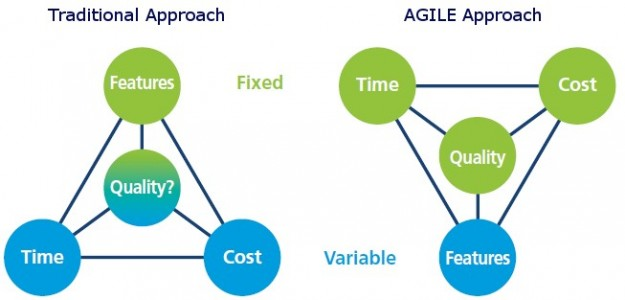
\includegraphics[scale=0.7]{Imagens/Traditional-Vs-Agile-e1409736279325.jpg}
    \caption{Comparação entre os Métodos Tradicionais e Métodos Ágeis}
    \label{fig:compta}
\end{figure}


\newpage

\subsection{Metodologia de Diagnóstico}

\begin{framed}
\noindent\textbf{Metodologia de Diagnóstico de um Projeto Ágil}
\qquad
Versão 1.0
\vspace{2mm}
\newline Este método de diagnóstico deve ser usado na fase de pré-planeamento de um projeto e servirá como uma escolha inicial entre os métodos mais tradicionais e um método Ágil. A primeira versão deste questionário apenas serve para indicar se deve ou não ser usada uma Metodologia Ágil, o método Ágil em específico não é tido em conta.
\vspace{1mm}
\newline Este questionário é constituído por 12 perguntas. As perguntas podem ter cotação 1, 2 ou 3 o que mede a sua importância e serve como fator multiplicativo.
\vspace{5mm}
\newline\textbf{Questão 1 - } Há uma necessidade dentro da sua organização de mudar de método de desenvolvimento?
\newline \begin{center} Sim \hspace{30mm} Não \end{center}
\vspace{2mm}
\newline\textbf{Questão 2 - } O projeto tem urgência e os prazos para sua conclusão são apertados?
\newline \begin{center} Sim \hspace{30mm} Não\end{center}
\vspace{2mm}
\newline\textbf{Questão 3 - } A sua equipa é bastante organizada?
\newline \begin{center} Sim \hspace{30mm} Não \end{center}
\vspace{2mm}
\newline\textbf{Questão 4 - } O cliente necessita de documentação clara de cada ciclo de desenvolvimento?
\newline \begin{center} Sim \hspace{30mm} Não \end{center}
\vspace{2mm}
\newline\textbf{Questão 5 - } O cliente necessita de aprovar o projeto a cada fase de desenvolvimento?
\newline \begin{center} Sim \hspace{30mm} Não \end{center}
\vspace{2mm}
\newline\textbf{Questão 6 - } O cliente está mais habituado e prefere usar métodos de desenvolvimento mais tradicionais?
\newline \begin{center} Sim  \hspace{30mm} Não\end{center}
\newline\textbf{Questão 7 - } Na sua perspetiva e mediante os projetos que a sua organização costuma trabalhar, qual é o tamanho do projeto?
\newline \begin{center} Pequeno \hspace{17mm} Médio\hspace{17mm}Grande\end{center}
\vspace{2mm}
\newline\textbf{Questão 8 - } São necessárias múltiplas variantes do projeto, ou pelo menos, são desejáveis?
\newline \begin{center} Sim\hspace{30mm} Não\end{center}
\vspace{2mm}
\newline\textbf{Questão 9 - } Qual é a área do projeto?
\newline \begin{center} Software ou Hardware \hspace{17mm} Serviços Financeiros \hspace{17mm}Serviços Profissionais \hspace{17mm} Outros\end{center}
\vspace{2mm}
\newline\textbf{Questão 10 - } O projeto está bem documentado e todos os requisitos estão definidos à partida?
\newline \begin{center} Sim \hspace{30mm} Não\end{center}
\vspace{2mm}
\newline\textbf{Questão 11 - } O cliente terá uma participação ativa no desenvolvimento do produto?
\newline \begin{center} Sim \hspace{30mm} Não \end{center}
\vspace{2mm}
\newline\textbf{Questão 12 - } Os elementos da sua equipa são pró-ativos e demonstram iniciativa?
\newline \begin{center} Sim \hspace{30mm} Não\end{center}
\vspace{10mm}

\vspace{10mm}
\begin{center}
\begin{itemize}
    \item \textbf{Menos de 10 pontos} - Os Métodos Ágil \\não são, à partida, apropriados ao seu projeto.
    \item \textbf{Entre 10 e 15 pontos} - Os Métodos Ágil talvez \\sejam apropriados mas necessita de uma segunda opinião.
    \item \textbf{Mais de 15 pontos} - Os Métodos Ágil são\\ apropriados ao seu projeto.
\end{itemize}
\end{center}
\end{framed}

\begin{table}[]
\centering
\label{my-label}
\begin{tabular}{|l|l|l|l|l|}
\hline
Pergunta/Pontuação & 0 pontos & 1 ponto                                                              & 2 pontos                                                           & 3 pontos                                                           \\ \hline
Pergunta 1         & Não      & Sim                                                                  & -                                                                  & -                                                                  \\ \hline
Pergunta 2         & Não      & -                                                                    & Sim                                                                & -                                                                  \\ \hline
Pergunta 3         & Não      & Sim                                                                  & -                                                                  & -                                                                  \\ \hline
Pergunta 4         & Sim      & -                                                                    & Não                                                                & -                                                                  \\ \hline
Pergunta 5         & Sim      & Não                                                                  & -                                                                  & -                                                                  \\ \hline
Pergunta 6         & Sim      & -                                                                    & Não                                                                & -                                                                  \\ \hline
Pergunta 7         & Grande   & Médio                                                                & Pequeno                                                            & -                                                                  \\ \hline
Pergunta 8         & Não      & Sim                                                                  & -                                                                  & -                                                                  \\ \hline
Pergunta 9         & Outros   & \begin{tabular}[c]{@{}l@{}}Serviços \\ \\ Profissionais\end{tabular} & \begin{tabular}[c]{@{}l@{}}Serviços \\ \\ Financeiros\end{tabular} & \begin{tabular}[c]{@{}l@{}}Software ou \\ \\ Hardware\end{tabular} \\ \hline
Pergunta 10        & Sim      & -                                                                    & Não                                                                & -                                                                  \\ \hline
Pergunta 11        & Não      & Sim                                                                  & -                                                                  & -                                                                  \\ \hline
Pergunta 12        & Não      & Sim                                                                  & -                                                                  & -                                                                  \\ \hline
\end{tabular}
\end{table}
